\documentclass{standalone}
\usepackage{tikz}
\usetikzlibrary{patterns, positioning}
\usepackage[sfdefault]{ClearSans} %% option 'sfdefault' activates Clear Sans as the default text font
\usepackage[T1]{fontenc}

\begin{document}
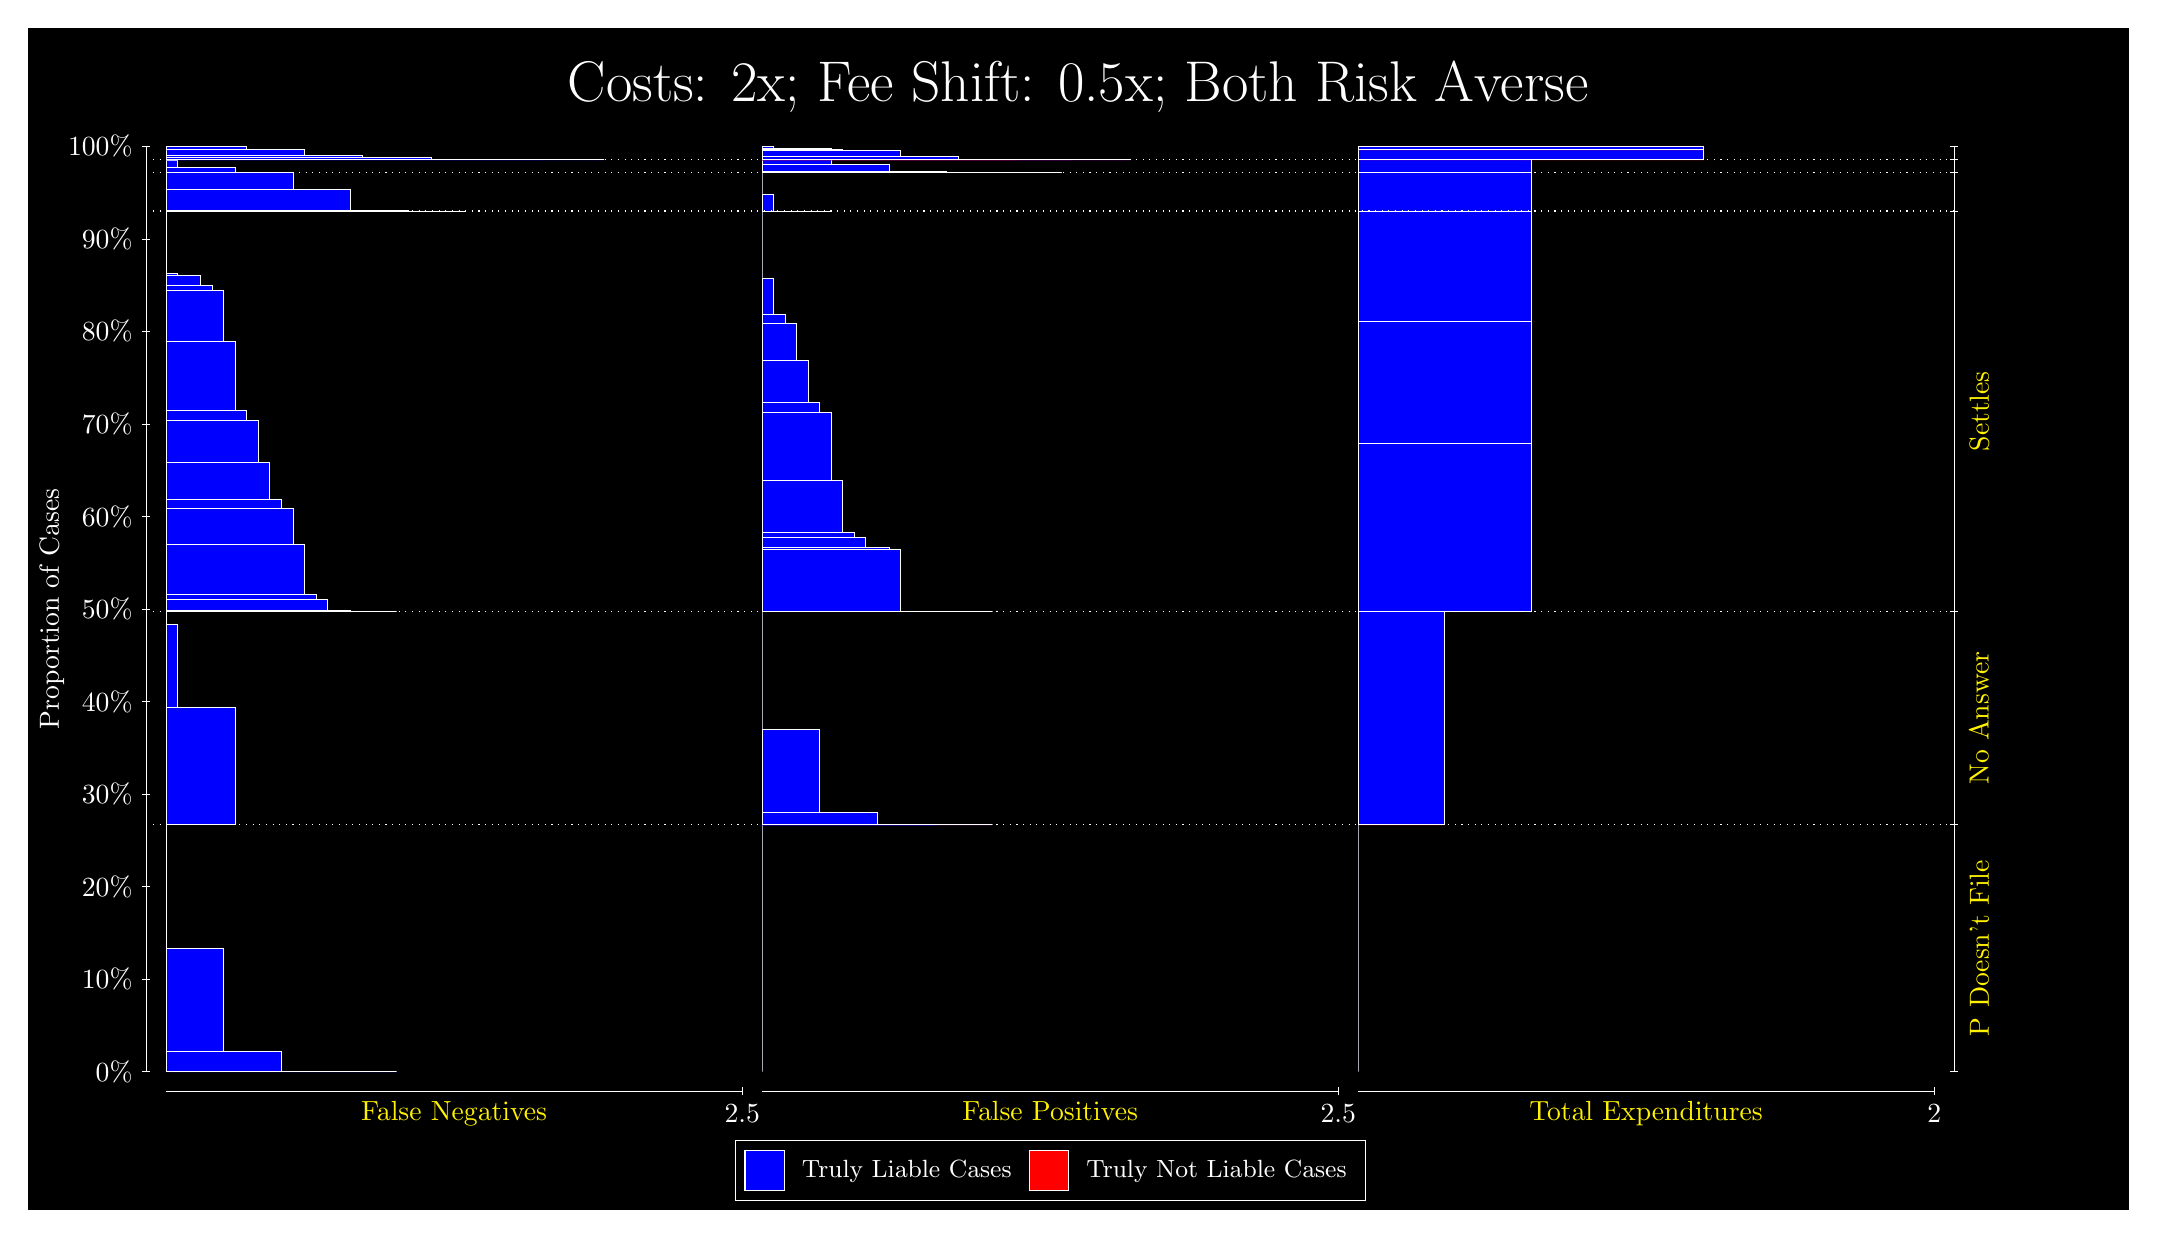
\begin{tikzpicture}
\draw[fill=black] (0,0) rectangle (26.667,15);
\draw[text=white] (0,13.5) rectangle (26.667,15) node[midway] {\huge Costs: 2x; Fee Shift: 0.5x; Both Risk Averse};
\draw[white, very thin] (1.5,1.75) -- (1.5,13.5);
\node[rotate=90, text=white, anchor=center] at (0.3, 7.625) {Proportion of Cases};
\draw[white, very thin] (1.45,1.75) -- (1.55,1.75);
\node[text=white, anchor=east] at (1.45, 1.75) {0\%};
\draw[white, very thin] (1.45,2.925) -- (1.55,2.925);
\node[text=white, anchor=east] at (1.45, 2.925) {10\%};
\draw[white, very thin] (1.45,4.1) -- (1.55,4.1);
\node[text=white, anchor=east] at (1.45, 4.1) {20\%};
\draw[white, very thin] (1.45,5.275) -- (1.55,5.275);
\node[text=white, anchor=east] at (1.45, 5.275) {30\%};
\draw[white, very thin] (1.45,6.45) -- (1.55,6.45);
\node[text=white, anchor=east] at (1.45, 6.45) {40\%};
\draw[white, very thin] (1.45,7.625) -- (1.55,7.625);
\node[text=white, anchor=east] at (1.45, 7.625) {50\%};
\draw[white, very thin] (1.45,8.8) -- (1.55,8.8);
\node[text=white, anchor=east] at (1.45, 8.8) {60\%};
\draw[white, very thin] (1.45,9.975) -- (1.55,9.975);
\node[text=white, anchor=east] at (1.45, 9.975) {70\%};
\draw[white, very thin] (1.45,11.15) -- (1.55,11.15);
\node[text=white, anchor=east] at (1.45, 11.15) {80\%};
\draw[white, very thin] (1.45,12.325) -- (1.55,12.325);
\node[text=white, anchor=east] at (1.45, 12.325) {90\%};
\draw[white, very thin] (1.45,13.5) -- (1.55,13.5);
\node[text=white, anchor=east] at (1.45, 13.5) {100\%};

\draw[white, very thin] (24.457,1.75) -- (24.457,13.5);
\draw[white, very thin] (24.407,1.75) -- (24.507,1.75);
\node[anchor=west] at (24.407, 1.75) {};
\draw[white, very thin] (24.407,4.8842) -- (24.507,4.8842);
\node[anchor=west] at (24.407, 4.8842) {};
\draw[white, very thin] (24.407,7.5931) -- (24.507,7.5931);
\node[anchor=west] at (24.407, 7.5931) {};
\draw[white, very thin] (24.407,12.678) -- (24.507,12.678);
\node[anchor=west] at (24.407, 12.678) {};
\draw[white, very thin] (24.407,13.17) -- (24.507,13.17);
\node[anchor=west] at (24.407, 13.17) {};
\draw[white, very thin] (24.407,13.331) -- (24.507,13.331);
\node[anchor=west] at (24.407, 13.331) {};
\draw[white, very thin] (24.407,13.5) -- (24.507,13.5);
\node[anchor=west] at (24.407, 13.5) {};

\draw[white, very thin, fill=blue] (1.75,1.75) rectangle (4.6775,1.75);
\draw[white, very thin, fill=blue] (1.75,1.75) rectangle (3.9457,1.7524);
\draw[white, very thin, fill=blue] (1.75,1.7524) rectangle (3.2138,2.002);
\draw[white, very thin, fill=blue] (1.75,2.002) rectangle (2.4819,3.32);
\draw[white, very thin, fill=red] (1.75,3.32) rectangle (1.75,3.32);
\draw[white, very thin, fill=blue] (1.75,3.32) rectangle (1.75,4.8842);
\draw[white, very thin, fill=blue] (1.75,4.8842) rectangle (2.6283,6.3772);
\draw[white, very thin, fill=blue] (1.75,6.3772) rectangle (1.8964,7.4336);
\draw[white, very thin, fill=red] (1.75,7.4336) rectangle (1.75,7.4336);
\draw[white, very thin, fill=blue] (1.75,7.4336) rectangle (1.75,7.5931);
\draw[white, very thin, fill=blue] (1.75,7.5931) rectangle (4.6775,7.5931);
\draw[white, very thin, fill=blue] (1.75,7.5931) rectangle (4.3848,7.5932);
\draw[white, very thin, fill=blue] (1.75,7.5932) rectangle (4.092,7.6062);
\draw[white, very thin, fill=blue] (1.75,7.6062) rectangle (3.9457,7.6067);
\draw[white, very thin, fill=blue] (1.75,7.6067) rectangle (3.7993,7.7455);
\draw[white, very thin, fill=blue] (1.75,7.7455) rectangle (3.6529,7.8081);
\draw[white, very thin, fill=blue] (1.75,7.8081) rectangle (3.5065,8.4507);
\draw[white, very thin, fill=blue] (1.75,8.4507) rectangle (3.3602,8.9072);
\draw[white, very thin, fill=blue] (1.75,8.9072) rectangle (3.2138,9.0178);
\draw[white, very thin, fill=blue] (1.75,9.0178) rectangle (3.0674,9.4929);
\draw[white, very thin, fill=blue] (1.75,9.4929) rectangle (2.921,10.025);
\draw[white, very thin, fill=blue] (1.75,10.025) rectangle (2.7746,10.153);
\draw[white, very thin, fill=blue] (1.75,10.153) rectangle (2.6283,11.018);
\draw[white, very thin, fill=blue] (1.75,11.018) rectangle (2.4819,11.677);
\draw[white, very thin, fill=blue] (1.75,11.677) rectangle (2.3355,11.735);
\draw[white, very thin, fill=blue] (1.75,11.735) rectangle (2.1891,11.861);
\draw[white, very thin, fill=blue] (1.75,11.861) rectangle (2.0428,11.862);
\draw[white, very thin, fill=blue] (1.75,11.862) rectangle (1.8964,11.894);
\draw[white, very thin, fill=red] (1.75,11.894) rectangle (1.75,11.894);
\draw[white, very thin, fill=blue] (1.75,11.894) rectangle (1.75,12.678);
\draw[white, very thin, fill=blue] (1.75,12.678) rectangle (5.5558,12.678);
\draw[white, very thin, fill=blue] (1.75,12.678) rectangle (4.8239,12.683);
\draw[white, very thin, fill=blue] (1.75,12.683) rectangle (4.092,12.955);
\draw[white, very thin, fill=blue] (1.75,12.955) rectangle (3.3602,13.168);
\draw[white, very thin, fill=blue] (1.75,13.168) rectangle (2.6283,13.17);
\draw[white, very thin, fill=red] (1.75,13.17) rectangle (1.75,13.17);
\draw[white, very thin, fill=blue] (1.75,13.17) rectangle (2.6283,13.231);
\draw[white, very thin, fill=blue] (1.75,13.231) rectangle (1.8964,13.323);
\draw[white, very thin, fill=red] (1.75,13.323) rectangle (1.75,13.323);
\draw[white, very thin, fill=blue] (1.75,13.323) rectangle (1.75,13.331);
\draw[white, very thin, fill=blue] (1.75,13.331) rectangle (7.3123,13.331);
\draw[white, very thin, fill=blue] (1.75,13.331) rectangle (6.5805,13.331);
\draw[white, very thin, fill=blue] (1.75,13.331) rectangle (5.8486,13.335);
\draw[white, very thin, fill=blue] (1.75,13.335) rectangle (5.7022,13.335);
\draw[white, very thin, fill=blue] (1.75,13.335) rectangle (5.1167,13.357);
\draw[white, very thin, fill=blue] (1.75,13.357) rectangle (4.9703,13.357);
\draw[white, very thin, fill=blue] (1.75,13.357) rectangle (4.3848,13.363);
\draw[white, very thin, fill=blue] (1.75,13.363) rectangle (4.2384,13.38);
\draw[white, very thin, fill=blue] (1.75,13.38) rectangle (3.6529,13.38);
\draw[white, very thin, fill=blue] (1.75,13.38) rectangle (3.5065,13.459);
\draw[white, very thin, fill=blue] (1.75,13.459) rectangle (2.921,13.459);
\draw[white, very thin, fill=blue] (1.75,13.459) rectangle (2.7746,13.498);
\draw[white, very thin, fill=blue] (1.75,13.498) rectangle (2.0428,13.5);
\draw[white, very thin, fill=red] (1.75,13.5) rectangle (1.75,13.5);
\draw[white, very thin, fill=blue] (1.75,13.5) rectangle (1.75,13.5);
\draw[white, very thin, fill=red] (9.3189,1.75) rectangle (9.3189,1.75);
\draw[white, very thin, fill=blue] (9.3189,1.75) rectangle (9.3189,4.8842);
\draw[white, very thin, fill=red] (9.3189,4.8842) rectangle (12.246,4.8842);
\draw[white, very thin, fill=blue] (9.3189,4.8842) rectangle (12.246,4.8842);
\draw[white, very thin, fill=blue] (9.3189,4.8842) rectangle (11.515,4.8844);
\draw[white, very thin, fill=blue] (9.3189,4.8844) rectangle (10.783,5.0436);
\draw[white, very thin, fill=blue] (9.3189,5.0436) rectangle (10.051,6.1001);
\draw[white, very thin, fill=blue] (9.3189,6.1001) rectangle (9.3189,7.5931);
\draw[white, very thin, fill=red] (9.3189,7.5931) rectangle (12.246,7.5931);
\draw[white, very thin, fill=blue] (9.3189,7.5931) rectangle (12.246,7.5931);
\draw[white, very thin, fill=red] (9.3189,7.5931) rectangle (11.954,7.5931);
\draw[white, very thin, fill=blue] (9.3189,7.5931) rectangle (11.954,7.5931);
\draw[white, very thin, fill=red] (9.3189,7.5931) rectangle (11.661,7.5931);
\draw[white, very thin, fill=blue] (9.3189,7.5931) rectangle (11.661,7.5931);
\draw[white, very thin, fill=blue] (9.3189,7.5931) rectangle (11.515,7.5931);
\draw[white, very thin, fill=red] (9.3189,7.5931) rectangle (11.368,7.5931);
\draw[white, very thin, fill=blue] (9.3189,7.5931) rectangle (11.368,7.5943);
\draw[white, very thin, fill=blue] (9.3189,7.5943) rectangle (11.222,7.5944);
\draw[white, very thin, fill=red] (9.3189,7.5944) rectangle (11.075,7.5944);
\draw[white, very thin, fill=blue] (9.3189,7.5944) rectangle (11.075,8.3765);
\draw[white, very thin, fill=blue] (9.3189,8.3765) rectangle (10.929,8.4088);
\draw[white, very thin, fill=blue] (9.3189,8.4088) rectangle (10.783,8.4101);
\draw[white, very thin, fill=blue] (9.3189,8.4101) rectangle (10.636,8.5355);
\draw[white, very thin, fill=blue] (9.3189,8.5355) rectangle (10.49,8.5942);
\draw[white, very thin, fill=blue] (9.3189,8.5942) rectangle (10.344,9.2529);
\draw[white, very thin, fill=blue] (9.3189,9.2529) rectangle (10.197,10.117);
\draw[white, very thin, fill=blue] (9.3189,10.117) rectangle (10.051,10.246);
\draw[white, very thin, fill=blue] (9.3189,10.246) rectangle (9.9044,10.778);
\draw[white, very thin, fill=blue] (9.3189,10.778) rectangle (9.758,11.253);
\draw[white, very thin, fill=blue] (9.3189,11.253) rectangle (9.6116,11.364);
\draw[white, very thin, fill=blue] (9.3189,11.364) rectangle (9.4652,11.82);
\draw[white, very thin, fill=blue] (9.3189,11.82) rectangle (9.3189,12.678);
\draw[white, very thin, fill=red] (9.3189,12.678) rectangle (10.197,12.678);
\draw[white, very thin, fill=blue] (9.3189,12.678) rectangle (10.197,12.68);
\draw[white, very thin, fill=blue] (9.3189,12.68) rectangle (9.4652,12.893);
\draw[white, very thin, fill=blue] (9.3189,12.893) rectangle (9.3189,13.17);
\draw[white, very thin, fill=red] (9.3189,13.17) rectangle (13.125,13.17);
\draw[white, very thin, fill=blue] (9.3189,13.17) rectangle (13.125,13.17);
\draw[white, very thin, fill=blue] (9.3189,13.17) rectangle (12.393,13.17);
\draw[white, very thin, fill=blue] (9.3189,13.17) rectangle (11.661,13.178);
\draw[white, very thin, fill=blue] (9.3189,13.178) rectangle (10.929,13.271);
\draw[white, very thin, fill=blue] (9.3189,13.271) rectangle (10.197,13.331);
\draw[white, very thin, fill=red] (9.3189,13.331) rectangle (14.003,13.331);
\draw[white, very thin, fill=blue] (9.3189,13.331) rectangle (14.003,13.331);
\draw[white, very thin, fill=red] (9.3189,13.331) rectangle (13.271,13.331);
\draw[white, very thin, fill=blue] (9.3189,13.331) rectangle (13.271,13.331);
\draw[white, very thin, fill=red] (9.3189,13.331) rectangle (12.539,13.331);
\draw[white, very thin, fill=blue] (9.3189,13.331) rectangle (12.539,13.333);
\draw[white, very thin, fill=blue] (9.3189,13.333) rectangle (11.807,13.372);
\draw[white, very thin, fill=red] (9.3189,13.372) rectangle (11.807,13.372);
\draw[white, very thin, fill=blue] (9.3189,13.372) rectangle (11.807,13.372);
\draw[white, very thin, fill=red] (9.3189,13.372) rectangle (11.661,13.372);
\draw[white, very thin, fill=blue] (9.3189,13.372) rectangle (11.661,13.372);
\draw[white, very thin, fill=blue] (9.3189,13.372) rectangle (11.075,13.451);
\draw[white, very thin, fill=blue] (9.3189,13.451) rectangle (11.075,13.451);
\draw[white, very thin, fill=red] (9.3189,13.451) rectangle (10.929,13.451);
\draw[white, very thin, fill=blue] (9.3189,13.451) rectangle (10.929,13.451);
\draw[white, very thin, fill=blue] (9.3189,13.451) rectangle (10.344,13.46);
\draw[white, very thin, fill=blue] (9.3189,13.46) rectangle (10.344,13.468);
\draw[white, very thin, fill=blue] (9.3189,13.468) rectangle (10.197,13.474);
\draw[white, very thin, fill=red] (9.3189,13.474) rectangle (10.197,13.474);
\draw[white, very thin, fill=blue] (9.3189,13.474) rectangle (10.197,13.474);
\draw[white, very thin, fill=blue] (9.3189,13.474) rectangle (9.6116,13.474);
\draw[white, very thin, fill=blue] (9.3189,13.474) rectangle (9.6116,13.474);
\draw[white, very thin, fill=blue] (9.3189,13.474) rectangle (9.4652,13.496);
\draw[white, very thin, fill=blue] (9.3189,13.496) rectangle (9.4652,13.496);
\draw[white, very thin, fill=blue] (9.3189,13.496) rectangle (9.3189,13.5);
\draw[white, very thin, fill=red] (16.888,1.75) rectangle (16.888,1.75);
\draw[white, very thin, fill=blue] (16.888,1.75) rectangle (16.888,4.8842);
\draw[white, very thin, fill=red] (16.888,4.8842) rectangle (17.986,4.8842);
\draw[white, very thin, fill=blue] (16.888,4.8842) rectangle (17.986,7.5931);
\draw[white, very thin, fill=red] (16.888,7.5931) rectangle (19.083,7.5931);
\draw[white, very thin, fill=blue] (16.888,7.5931) rectangle (19.083,9.7314);
\draw[white, very thin, fill=red] (16.888,9.7314) rectangle (19.083,9.7314);
\draw[white, very thin, fill=blue] (16.888,9.7314) rectangle (19.083,11.283);
\draw[white, very thin, fill=red] (16.888,11.283) rectangle (19.083,11.283);
\draw[white, very thin, fill=blue] (16.888,11.283) rectangle (19.083,12.678);
\draw[white, very thin, fill=red] (16.888,12.678) rectangle (19.083,12.678);
\draw[white, very thin, fill=blue] (16.888,12.678) rectangle (19.083,13.17);
\draw[white, very thin, fill=red] (16.888,13.17) rectangle (19.083,13.17);
\draw[white, very thin, fill=blue] (16.888,13.17) rectangle (19.083,13.331);
\draw[white, very thin, fill=red] (16.888,13.331) rectangle (21.279,13.331);
\draw[white, very thin, fill=blue] (16.888,13.331) rectangle (21.279,13.459);
\draw[white, very thin, fill=red] (16.888,13.459) rectangle (21.279,13.459);
\draw[white, very thin, fill=blue] (16.888,13.459) rectangle (21.279,13.5);
\draw[white, dotted] (1.5,4.8842) -- (24.457,4.8842);
\draw[white, dotted] (1.5,7.5931) -- (24.457,7.5931);
\draw[white, dotted] (1.5,12.678) -- (24.457,12.678);
\draw[white, dotted] (1.5,13.17) -- (24.457,13.17);
\draw[white, dotted] (1.5,13.331) -- (24.457,13.331);
\draw[white, very thin] (1.75,1.5) -- (9.0689,1.5);
\node[text=yellow, anchor=north] at (5.4094, 1.5) {False Negatives};
\draw[white, very thin] (9.0689,1.45) -- (9.0689,1.55);
\node[text=white, anchor=north] at (9.0689, 1.45) {2.5};

\draw[white, very thin] (9.3189,1.5) -- (16.638,1.5);
\node[text=yellow, anchor=north] at (12.978, 1.5) {False Positives};
\draw[white, very thin] (16.638,1.45) -- (16.638,1.55);
\node[text=white, anchor=north] at (16.638, 1.45) {2.5};

\draw[white, very thin] (16.888,1.5) -- (24.207,1.5);
\node[text=yellow, anchor=north] at (20.547, 1.5) {Total Expenditures};
\draw[white, very thin] (24.207,1.45) -- (24.207,1.55);
\node[text=white, anchor=north] at (24.207, 1.45) {2};

\node[text=yellow, centered, rotate=90] at (24.777, 3.3171) {P Doesn't File};
\node[text=yellow, centered, rotate=90] at (24.777, 6.2386) {No Answer};
\node[text=yellow, centered, rotate=90] at (24.777, 10.135) {Settles};




\draw (12.978300999999998,1.5) node[draw=none] (baseCoordinate) {};
\begin{scope}[align=center]
        \matrix[scale=0.5, draw=white, below=0.5cm of baseCoordinate, nodes={draw}, column sep=0.1cm]{
            \node[rectangle, draw, minimum width=0.5cm, minimum height=0.5cm, fill=blue] {}; &
            \node[draw=none, font=\small, text=white] (B) {Truly Liable Cases}; &
            \node[rectangle, draw, minimum width=0.5cm, minimum height=0.5cm, fill=red] {}; &
            \node[draw=none, font=\small, text=white] (B) {Truly Not Liable Cases}; \\
            };
\end{scope}

\end{tikzpicture}
\end{document}